\chapter{Teorie}

Semestrální práce se zejména zabývá problematikou \acs{MIR}. Popsánou v kapitole (!doplnit kapitolu!).
Důležitou roli zde hraje i úvaha nad realizací světelných animací.
Je důležité aby bylo přemýšleno nad principem reakce světelných animací na hudbu.
Nabízejí se otázky jak by měla daná animace reagovat na konkrétní děj skladby.
Jakým způsobem navrhnout strukturu \dots

V táto části je popsána teorie zpracování hudební nahrávky pomocí známých algoritmů jako je například \acs{FFT} (\acl{FFT}) 
či nabízené možnosti strojového učení. Struktura a možnosti systému Spectoda pro generování interaktivních světelných animací.
Uměleckou částí, jak by měla animace prezentovat hudbu.

\section{MIR - Music information retrieval}
    Music information retrieval je interdisciplinární vědní obor sostředící se na získávání infromací z hudebních nahrávek.
    Jsou zde kombinovány znalosti mnoha oborů jako jsou muzikologie, psychoakustika, strojové učení, zpracování signálů a další.
    
    Výstup jeho výzkumu je využíván populárními technologiemi. 
    Jednou z aplikací je personalizované doporučování hudebních skladeb, která se nachází v moderních streamovacích platformách.
    Další využítí je v programech pro mixování hudby používaných diskžokeji k plynulejší práci díky alanýze tempe a klíčových částí skladby.
    Tyto technologie se nachází v mnoha dalších aplikacích a s šířením se digitálního audia jejich důležitost stále poroste.

    V \acs{MIR} jako vstupní data využívají zejména hudební informace v digitální potobě.
    Tyto data se rozlišují do více typů. Mohou to být obrázky představující digitální formu zápisu hudby pomocí symbolů (not).
    Dalším možným typem je "digitální hudba", představovaná zápisem v \acs{MIDI} notách.
    V této práci budou jako vstupní data yvužívány digitální hudební nahrávky ("digitální audio"). 
    
    Pipeline - řetězec zpracování (TODO: najít vhodné slovíčko v češtině)

    Téměř standardně využívaný řetězec procesů v aplikacíc \acs{MIR} je popsána níže. 
    Pokud jsou vstupní data komplexní na začátku je v řetězci zařezen blok předzpracování, která se stará o komprimaci vstupních singálů.
    U hudebních signálů se jedná například o konverzi stereo signálů na mono signál a jeho následnou komprimaci popsanou více v bodě (TODO: odkaz na bod audio)
    Dalším bodem v řetězci je extrakce vlastností signálu. 
    Zde je je nastaven poměr mezi vlastnostmi důležitými pro strojové učení lidskou expertní znalost.
    Poměr mezi těmito vlastnostmi závisí na aplikaci pro kterou je algoritmus určen.
    Ná základě získaných vlastností je nastavena struktura algoritmu pro odvození výsldných parametrů.
    (Popsat víc + přidat schéma z knihy strana 213-224)
\cite{BurgoyneJohnAshley2015MIR}

\begin{figure}[!h]
    \centering
    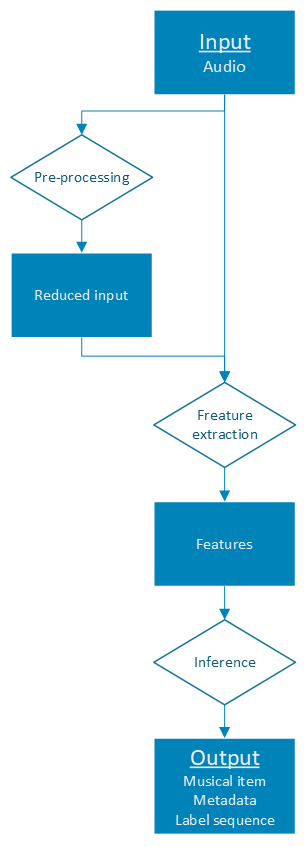
\includegraphics[width = 0.4\linewidth]{obrazky/MIR-diagram.png}
    \caption{Řetězec procesů MIR \cite{BurgoyneJohnAshley2015MIR}}
    \label{fig:MIR_diagram}
\end{figure}

    Zpracování audio signálů je již dvě desetilétí hlavním trendem výzkumu \acs*{MIR}.
    Je to přirození tím, že zde není téměř žádná přirozená hranice a je možné téměř vše.
    Právní podmínky jsou zde příznivé a vědecké instituce nemají problém pro svou práci získat velké množství materiálu chráněného autorským právem.
    Z důvodu velké komplexsnosti vstupních signálů se využívá několik technik komprimaca signálů kterými jsou. 
    Slučování vícekanálových nahrávek do mono sginálu. Převzorkování signálu na nižší vzorkovací kmitočty,
    a rozložení signálu na krátké překrývající se úseky ze kterých mohou být nezávisle extrahovány jejich vlastnosti. 
    Výsledkem je kolekce paralelně složených sekvencí hodnot vlastností, které se následně použijí pro odvozování (inference).

  \begin{table}[!h]
    \centering
    \begin{tabular}{|p{0.07\linewidth} | p{0.31\linewidth} | p{0.27\linewidth} | p{0.25\linewidth}|}
        \hline
        {\bf Data}                 & {\bf Vyhledávání informací} & {\bf Klasifikace a odhad} & {\bf Sekvenční značení}\\
        \hline
        Audio                      & Identifikace skladby,
                                     Řazení,
                                     Měření podobnosti,
                                     Získání otisku,
                                     Generování seznamu skladeb
                                   & Identifikace umělce a skladatele,
                                     Žánr a nálada,
                                     Určení tempa
                                   & Extrakce melodie,
                                     Odhad akordů,
                                     Detekce nástupů,
                                     Segmentace                   \\
        \hline
    \end{tabular}
    \caption{Typické procesy na základně vstupních a výstupních dat.}
    \label{tab:MIR_typicke_procesy}
  \end{table}

\subsection{Beat and tempo detection}

\subsection{Parametrizace hudebních signálů}

\section{Systém Spectoda}

\section{Hudební signál jako animace}